%!TEX encoding=UTF-8
%!TEX program=xelatex
\documentclass{./source/Report}

\newtheorem{problem}{Problem}
\newtheorem{definition}{Definition}

\begin{document}

\title{Quantum Approximate Optimization Algorithm(QAOA)}

\author{Qin Yuyang, Ren Tingxu, Chen Ke, Lai Pengyi}
\affiliation{CKC  College  Zhejiang  University, Hangzhou  310058}

\date{\today}

\begin{abstract}
Quantum Approximate Optimization Algorithm is a hybrid quantum-classical algorithm for solving combinatorial optimization problems. The depth $p$ and the chosen parameters can greatly influence the algorithm's performance. Based on related papers, we implement unitary matrix operator simulation, deploy three methods to optimize $\vec{\gamma}, \vec{\beta}$ and compare their performance. Then we construct the quantum circuits and use qiskit SDK to simulate them. Besides, we test  our quantum circuits' performance under real IBM Quantum Machines noise. Lastly, We study the influence of $p$ on QAOA for a given graph, and lots of results are analyzed. Our codes are available at  \href{https://github.com/qyy2003/QAOA}{github}
\end{abstract}

\maketitle

\section{Background}
\subsection{Combinatorial Optimization Problem}
Given $n$ bits and $m$ clauses, the combinatorial optimization problem asks for a string $z=z_1z_2...z_n$ that maximize the cost function 
\begin{equation}
  C(z) = \sum_{\alpha=1}^mC_{\alpha}(z)
\end{equation}
where $C_{\alpha}=1$ if $z$ satisfies clause $\alpha$ and $0$ if it doesn't satisfies.
Usually, finding optimization solutions is hard and costly using classical algorithms, but it is relatively 
easier to achieve an approximate solution close to the maximum of $C(z)$. This kind of method is called 
approximate optimization algorithm.  The performance of an approximate optimization algorithm is guaranteed by an approximate ratio of $R$
such that 
\begin{equation}
    \frac{C(z)}{\max_{z}C(z)}\ge R
\end{equation}

\subsection{Maximum Cut}

\begin{problem}[Maximum Cut (MaxCut)]
Given a graph $G =(V, E)$ with $n$ vertices and $m$ weighted edges, separate 
$V$ into two disjoint sets $S$ and $T$ to maximize the sum of weights of edges $(u, v)$ 
such that $u\in S, v\in T$ or $v\in S, u\in T$.
\end{problem}

The MaxCut problem is a well-known combinatorial optimization 
problem. The problem is NP-hard and APX-hard, meaning that no polynomial-time 
algorithm has been found and the approximate ratio obtained by polynomial-time algorithms
cannot be arbitrarily close to the optimal solution unless $NP=P$. 

The quantum computer works under the $2^n$ dimensional Hilbert space. To solve the combinatorial optimization problem, 
it is expected to construct a Hamiltonian (phase Hamiltonian) $C$ such that
\begin{equation}
    C\ket{z}=C(z)\ket{z}
    \label{eq:parallelism}
\end{equation}
where $\ket{z}$ is a base in computational basis. In this way, the problem of finding the maximum of $C(z)$ changes into finding the extremal eigenvalue for the phase Hamiltonian.

\begin{definition}[Phase Hamiltonian]
The phase Hamiltonian for the MaxCut problem is constructed as
\begin{equation}
    C=\sum_{\langle jk\rangle}\frac{w_{jk}}{2}(1-\sigma_j^z\sigma_k^z)
\end{equation}
where $w_{jk}$ is the weight of edge $\langle jk \rangle$.
\end{definition}
Let's take the $2^2$ dimensional Hilbert space as an example to see how this construction works.
If there is an edge between the two vertices, then 
\begin{equation}
    \sigma_0^z\sigma_1^z = 
    \left( \begin{matrix}
        1 & 0 & 0 & 0 \\ 0 & -1 & 0 & 0 \\ 0 & 0 & -1 & 0 \\ 0 & 0 & 0 & 1
    \end{matrix} \right)
\end{equation}
\begin{equation}
    C = \frac{w}{2}(1-\sigma_0^z\sigma_1^z)=
    \left( \begin{matrix}
        0 & 0 & 0 & 0 \\ 0 & w & 0 & 0 \\ 0 & 0 & w & 0 \\ 0 & 0 & 0 & 0
    \end{matrix} \right)
\end{equation}

This means that the result of $C\vert z\rangle$ is equal to $w$ if and only if the two vertices 
are in different sets, i.e., $\vert z \rangle = \vert 01\rangle$ or $\vert z \rangle =\vert 10\rangle$. Taking the sum over all 
edges, we can prove that this construction satisfies Equation~\ref{eq:parallelism}.

\subsection{QAA: Quantum Adiabatic Algorithm}

Quantum Adiabatic Algorithm is a method raised around 2000 to solve combinatorial search problems~\cite{farhi2000quantum}. The algorithm 
begins with an initial state $|s\rangle$ which is the groudn state of $B$. Then it constructs a time-dependent Hamiltonian
\begin{equation}
    H(t)=(1-\frac{t}{T})B+\frac{t}{T}C 
\end{equation} 

Let the system evolve according to the Schrödinger equation for a sufficiently long time $T$. The system is expected to 
stay in the ground state over the smooth evolution. In the end, the ground state of $H(T) = C$ can be obtained.

However, in practical situations, the long evolution time can be intolerable. 
In addition, the energy levels change continuously over time $T$, and in some occasions, two 
energy levels may be pretty near or even cross each other. If this happens to the two lowest energy levels, 
the system will jump into the other energy level and leave the ground state. This means that a long-time evolution cannot guarantee
the maximum answer to be found. These drawbacks greatly limit the performance of QAA.

\section{Algorithm specification}

Quantum Approximate Optimization Algorithm (QAOA) uses 
a Trotterized approximation of QAA to obtain a quantum gate model algorithm~\cite{farhi2014quantum}.
It separates the continuous evolution process into countable stages and repeatedly applies the short-time evolution of the Phase Operator and the Mix operator to get a state similar to the desired ground state.

\subsection{Operator Definition}
\begin{definition}[Phase operator]
Define the Phase Operator as 
\begin{equation}
    U(C, \gamma)=e^{-i\gamma C}
\end{equation} 
\end{definition}
where $\gamma\in [0, 2\pi]$ because $C$ is a diagonal matrix with integar elements. 
The phase operator can be regarded as applying the Phase Hamiltonian for a short time proportion
to $\gamma$.

\begin{definition}[Mix Hamiltonian]
Define the Mix Hamiltonian as 
\begin{equation}
    B=\sum_{i=1}^n\sigma_i^x
\end{equation}
\end{definition}
This Hamiltonian is constructed for convenient preparation of the initial state. 
The ground state of this Hamiltonian is simply a sum over all computational basis
\begin{align*}
    |s\rangle = |+\rangle^{\oplus n}=\frac{1}{\sqrt{n}}\sum_z |z\rangle
\end{align*} 
Therefore, this ground state for $B$ is chosen as the initial state for the evolution.

\begin{definition}[Mix Operator]
Define the Mix Operator as 
\begin{align*}
    U(B, \beta)=e^{-i\beta B}
\end{align*} 
\end{definition}
where $\beta \in [0, \pi]$. Similar to the Phase Operator, this operator functions 
as applying the Mix Hamiltonian for a short time, which is proportioned to $\beta$. 

\subsection{Envolution}

Recall the process of QAA, the long evolution time can 
be cut into multiple small periods of time-independent evolution.
For a small time interval $\Delta t \hbar$ at time $t$, the evolution operator 
can be appropriated by 
\begin{equation}
    \begin{aligned}
   U \approx e^{-iH(t)\Delta t} &= e^{-i(uB+vC)\Delta t} \\
   &= \lim_{N\rightarrow \infty}(e^{-iuB\Delta t/N}e^{-ivC\Delta t/N})^N
    \end{aligned}
\end{equation}
where $u=(1-\frac{t}{T}), v=\frac{t}{T}$. 

Notice that the decomposition operators are just 
in the form of Phase operators or Mix operators, which inspires us to apply these two kinds of 
operators alternatively on the initial state. For a depth $p$ and $2p$ predetermined parameters 
$(\vec{\gamma}, \vec{\beta})$, define a quantum state.
\begin{equation}
    |\vec{\gamma}, \vec{\beta}\rangle=U(B,\beta_p)U(C,\gamma_p)...U(B,\beta_1)U(C,\gamma_1)|s\rangle 
\end{equation}

The expectation of eigenvalues of $C$ when we measure $|\vec{\gamma},\vec{\beta}\rangle$ in computational basis is
\begin{align*}
    F_p(\vec{\gamma}, \vec{\beta}) = \langle\vec{\gamma},\vec{\beta}| C |\vec{\gamma},\vec{\beta}\rangle
\end{align*}

For sufficiently large $p$ and appropriately chosen parameters, the state can evolve into the ground state
of $C$ as discussed above. Therefore, 
\begin{align*}
    \lim_{p\rightarrow \infty}\max_{\vec{\gamma}, \vec{\beta}}{F_p(\vec{\gamma}, \vec{\beta})}=C_{max}(z)
\end{align*}

In reality, we cannot make $p$ as large as infinity, but an approximate solution can be obtained using this 
state for finite $p$. To do this, repeatedly measure $|\vec{\gamma}, \vec{\beta}\rangle$ in computational basis. For each measure 
result $\vert z \rangle$, compute $C(z)$ using traditional computers and keep the maximum number of this value as $\hat{C}(z)$. Over many 
times of measurements, $\hat{C}(z)$ will be close to or greater than $ F_p(\vec{\gamma}, \vec{\beta})$. If we can optimize 
the parameters for this value, then an approximate optimization solution is found.


\section{Circuit Description}

\subsection{The Phase Operator}

The circuit for the Phase Operator $U(C, \gamma)$ varies over different problems and depends on the composition of $C$. 
For the MaxCut problem, $U(C, \gamma)$ can be decomposed into a unitary operator for each edge using Trotter decomposition.
Therefore, we can design the circuit separately for every edge.
\begin{align*}
    U(C, \gamma) &= e^{-i\gamma\sum_{\langle jk\rangle}C_{\langle jk\rangle}}\\
    &=\Pi_{\langle jk\rangle}e^{-i\gamma \frac{w}{2}(-\sigma_j^z\otimes\sigma_k^z+I)}\\
    &=\Pi_{\langle jk\rangle}e^{-i\frac{-\gamma w}{2}(\sigma_j^z\otimes\sigma_k^z)}e^{-i\frac{\gamma w}{2}I}
\end{align*}

$e^{-i\frac{-\gamma w}{2}(\sigma_j^z\otimes\sigma_k^z)}$ can be implemented as a CNOT gate, a z-rotation gate and another CNOT gate. 
while $e^{-i\frac{\gamma w}{2}I}$ is a z-rotation gate applied to $|0\rangle$.

Therefore, an edge $\langle jk\rangle$this operator can be implemented in the circuit like FIG.\ref{fig:uc}.

\begin{figure}
\begin{quantikz}
\lstick{$\ket{x_j}$} & \ctrl{1} & \qw                     & \ctrl{1} & \qw \\
\lstick{$\ket{x_k}$} & \targ{}  & \gate{R_Z(-\gamma w)}   & \targ{}  & \qw \\
\lstick{$\ket{0}$}   & \qw      & \gate{R_Z(-\gamma w/2)} & \qw      &
\end{quantikz}
\caption{Quantum circuit for an edge $\langle jk\rangle$ in the Phase Operator }
\label{fig:uc}
\end{figure}


\subsection{The Mix Operator}
The Mix Operator contains the sum of the $\sigma_x$ operator of each qubit.
\begin{equation}
    U(B, \beta) = e^{-i\beta\sum\sigma_i^x}
\end{equation}
Therefore, the circuit is to simply add an x-rotation gate $R_{2\beta}^X$ for each qubit as FIG.\ref{fig:ub}, where
\begin{align*}
    R_{\phi}^X=cos(\phi/2)I_2-sin(\phi/2)i\sigma_x
\end{align*}

\begin{figure}
\begin{quantikz}
\lstick{$\ket{x_1}$} & \gate{R_X(2\beta)} & \qw \\
\lstick{\vdots} \\
\lstick{$\ket{x_n}$} & \gate{R_X(2\beta)} & \qw 
\end{quantikz}
\caption{Quantum circuit for the Mix Operator}
\label{fig:ub}
\end{figure}

The overall circuit is a combination of these designs. 

\section{Optimizing}

A complete process for the QAOA algorithm of depth $p$ works as below:

\begin{enumerate}
    \item Choose a set of $2p$ parameters $(\vec{\gamma}, \vec{\beta})$ and use them to build the circuit
    \item Use quantum computer to get the state $\vec{\gamma}, \vec{\beta}\rangle$
    \item Measure the state in computational basis multiple times and record the resulting $|z\rangle$ with maximum $C(z)$ 
    \item Adjust parameters $(\gamma, \beta)$ and repeat steps 3 and 4 to get a better solution
    \item Output the maximum result
\end{enumerate}

The performance of QAOA greatly depends on the choice of $p$ and the parameters. Usually, $p$ is limited 
by the hardware and upstream algorithms. Therefore, how to find appropriate parameters to optimize the answer is a core problem.
This part is usually solved using classical optimization methods based on iteration. 
As a result, QAOA is divided into the category of hybrid quantum-classical algorithms.

\subsection{Optimizing methods}

The most brute force method is  to iterate over a fine grid over the $[0, 2\pi]^p \times [0, \pi]^p$
space. Supposing each interval is divided into $k$ segments, the time complexity will be as large as 
$O(k^{2p})$. However, the complexity is still independent of $n$, meaning that this method can still 
have some application in occasions with small depth.

Generally, the classical optimization method can be classified into two categories. 
One is gradient-based algorithms, the most classical of which is the gradient descent. 
In this kind of method, the way of finding the gradient at a given point also varies. These methods
may achieve different performances in different situations. The other category is the gradient-free algorithm.
In our experiment, we chose Bayesian Optimization as an example. Since the quantum computer 
can be regarded as a black box for upstream algorithms, there are a great many numerical analysis methods 
to undertake this work. As long as the search space is $[0, 2\pi]^p \times [0, \pi]^p$, the complexity 
can remain independent of $n$. This is where quantum methods differ from traditional algorithms for Combinatorial Optimization Problem.

When $p$ is relatively large, there are also some tricks we can perform on the initial value of 
$(\vec{\gamma}, \vec{\beta})$. For example, use the optimal values for smaller $p$ to interplot the parameters for larger $p$.
Similar methods can greatly reduce the number of iterations needed for follow-up optimization~\cite{Zhou_2020}.


\section{Experiment Design}
In this section we focus on how we design our experiment, implement it with our code, along with our code structure and some fixed bugs.

We focus on the optimization and simulation of the QAOA algorithm and its implementation on the Max-Cut problem in Python. First, we implement the QAOA utilizing the unitary matrix operator in numpy form. Then we use grid search, Bayesian Optimization and L-BFGS-B to find the best $\beta,\gamma$. With the best  $\beta,\gamma$, we construct its quantum circuits and simulate them both with and without noise using IBM qiskit SDK\cite{Qiskit}. 

\subsection{Data Preparation}
\begin{itemize}
    \item \textbf{graphic\_in.py}: To prepare a random graph with n nodes and get the Max-Cut classic result of it, where \textbf{generateGraph()}  could new a graph and \textbf{graphic(n, edge.ask\_min())} provides its Max-Cut answer as well as division scheme in hexadecimal. The graph will be saved into \textbf{grapy\_in.npy}. 
    \item \textbf{graphic\_print.py}: draw the graph using networkx SDK.
\end{itemize}

\subsection{Unitary Matrix Operator Simulation}
In the QAOA algorithm, we have 
\begin{align*}
    |\vec{\gamma}, \vec{\beta}\rangle=U(B,\beta_p)U(C,\gamma_p)...U(B,\beta_1)U(C,\gamma_1)|s\rangle 
\end{align*}
where 
\begin{align*}
    U(C, \gamma)=e^{-i\gamma C},U(B, \beta)=e^{-i\beta B}
\end{align*}
which could be achieved by our Python code. There are two methods, eigenvalue decomposition and \textbf{np.linalg.eigh} implementation.Eigenvalue decomposition is faster while \textbf{np.linalg.eigh} implementation get better results.


\subsubsection{Eigenvalue Decomposition}
If $C$ is a Hermitian matrix, then it can be diagonalized as $C = UDU^\dagger$, where $U$ is a unitary matrix and $D$ is a diagonal matrix with diagonal elements being the eigenvalues of $C$. Therefore, we can write $e^{-i\gamma C}$ as:
\begin{align*}
    e^{-i\gamma C} = e^{-i\gamma UDU^\dagger}
\end{align*}
Since $U$ is a unitary matrix, it satisfies $UU^\dagger = U^\dagger U = I$. According to the definition of matrix exponential function, we have:
\begin{align*}
    e^{-i\gamma UDU^\dagger} &= \sum_{n=0}^{\infty} \frac{(-i\gamma UDU^\dagger)^n}{n!}\\
    &= \sum_{n=0}^{\infty} \frac{(-i\gamma)^n (UDU^\dagger)^n}{n!}
\end{align*}
Since $U^\dagger U = I$, $(UDU^\dagger)^n = UD^nU^\dagger$. Therefore, we can write the above formula as:
\begin{align*}
    e^{-i\gamma UDU^\dagger} &= \sum_{n=0}^{\infty} \frac{(-i\gamma)^n UD^nU^\dagger}{n!} \\
    &= U\left(\sum_{n=0}^{\infty} \frac{(-i\gamma)^n D^n}{n!}\right)U^\dagger \\
    &= Ue^{-i\gamma D}U^\dagger
\end{align*}

Therefore, by performing eigenvalue decomposition on $C$, we can transform the calculation of the matrix exponential function into a direct calculation of diagonal elements. In this way, we can avoid the error of the matrix exponential function. However, the precision of eigenvalue decomposition obtained by \textbf{np.linalg.eig} cannot meet the requirements. Its error is so significant that the result of $e^{-i\gamma C}$ is no longer a unitary matrix anymore. By multiplying these so-called unitary matrices, the magnitude of the final state $|\vec{\gamma}, \vec{\beta}\rangle $ is far away from 1. It's the first \textbf{precision disasters} we have met. When we use tried different $\vec{\gamma}, \vec{\beta} $ in the optimization section to get the best parameters, sometimes we got dramatical results like $F_p$ larger than 10000.  To solve the problem, we finally discover this precision bug.  So we used \textbf{np.linalg.eigh} for eigenvalue decomposition to achieve better precision. 




\subsubsection{Expm Direct Calculation}
Since the method of eigenvalue decomposition doesn't work, we are forced to seek other solutions, which leads us to \textbf{scipy.linalg.expm}. We analyze its result, which turns out to be a nice one. We find $e^{-i\gamma C}$ is a unitary matrix and the magnitude of the final state $|\vec{\gamma}, \vec{\beta}\rangle $ is about 0.9999, which is a satisfactory result. So we choose the new method and solve the first \textbf{precision disasters}.

\subsection{Parameter Optimization}

Now, given an array of $|\vec{\gamma}, \vec{\beta}\rangle$, We could simulate the QAOA. So we try to find the best array of $|\vec{\gamma}, \vec{\beta}\rangle$ at fixed $p$. That's exactly what we do in \textbf{optimize.ipynb}, finding the best array of $|\vec{\gamma}, \vec{\beta}\rangle$ at fixed $p$ and n with various methods.

We use dfs to achieve the grid search, hyperopt package\cite{bergstra2013making} to finish Bayesian Optimization and scipy. optimize to implement the basin-hopping algorithm in the L-BFGS-B method. We compare these three algorithms using its $F_p$. 
\begin{align*}
    F_p(\vec{\gamma}, \vec{\beta}) = \langle\vec{\gamma},\vec{\beta}| C |\vec{\gamma},\vec{\beta}\rangle
\end{align*}

According to our test result shown as TABLE.\ref{tab:Opt}, it turns out that basin-hopping and L-BFGS-B have done a faster and better job. 

We want to find out how $F_p$ changes as $p$ increases in two fixed graphs shown as FIG.\ref{fig:n=7} and FIG.\ref{fig:n=8}. So we iterate $p$ in $range(1,11)$  and utilize the basin-hopping algorithm in the L-BFGS-B method to optimize the $F_p$  for each $p$. Then we get the result of each $p$ and save the $\vec{\gamma},\vec{\beta}$. And the formulation of accuracy we use here is 
\begin{align*}
    \text{Accuracy}=\frac{F_p(\vec{\gamma}, \vec{\beta})}{\text{Answer of classical Algorithm}}
\end{align*}


We tried to run as large n as possible. However, as n increases 1, the unitary matrix times 4 and it will take more attempts in the parameter fine-tuning process. At last, we chose n=8 and generate a graph as shown in FIG.\ref{fig:n=8}. We run on Lab's \textit{Intel(R) Xeon(R) Gold 6226R CPU @ 2.90GHz} and it takes us several days to get the final result.

\begin{figure}[!htb]
    \centering
    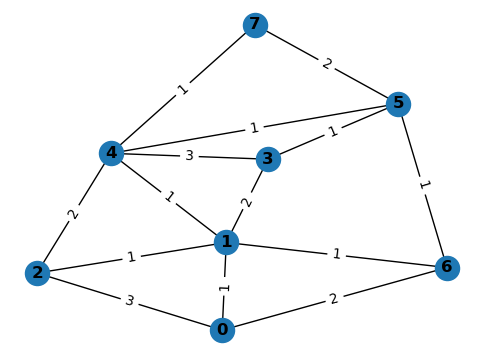
\includegraphics[width=0.309\textwidth]{graphic_n=8.png}
    \caption{An Graphic Example of n=8,whose Max Cut = 19}
    \label{fig:n=8}
\end{figure}

However, when we attempt to simulate the quantum circuit, we find out that we could only simulate a quantum circuit with noise in n=7 utilizing qiskit since the free IBM quantum machine has a maximum qubit of 7 and we use its noise data. Since quantum circuit simulation needs the optimized $\vec{\gamma},\vec{\beta}$, we generate a new graph, shown as FIG.\ref{fig:n=7}, and repeat the above process.

\begin{figure}[!htb]
    \centering
    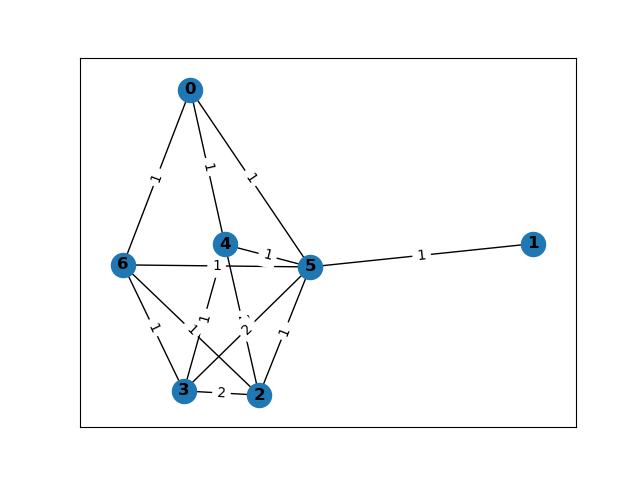
\includegraphics[width=0.309\textwidth]{graphic_n=7.png}
    \caption{An Graphic Example of n=7,whose Max Cut = 11}
    \label{fig:n=7}
\end{figure}

\clearpage

\subsection{Quantum Circuits Simulation}

We prepare our qubits with a Hadamard Gate to obtain the mixed state. $U(C, \gamma)=e^{-i\gamma C}$ could be achieved by applying a $Rz(-\gamma)$ and two $C_x$ gate at  both ends of it.  $U(B, \beta)=e^{-i\beta B}$ could be simply implemented deploying $R_x(2\beta)$ gate. In this way, we succeed in constructing the quantum circuit. Our code could be run on quantum machines, but the long waiting list prevents us. The typical quantum circuit our code generated is shown as FIG.\ref{fig:example circuit}. The datasheet of IBM nairobi, the real quantum machine we simulate, is shown in FIG.\ref{fig:overview of ibm_nairobi}.

\begin{figure}[!htb]
    \centering
    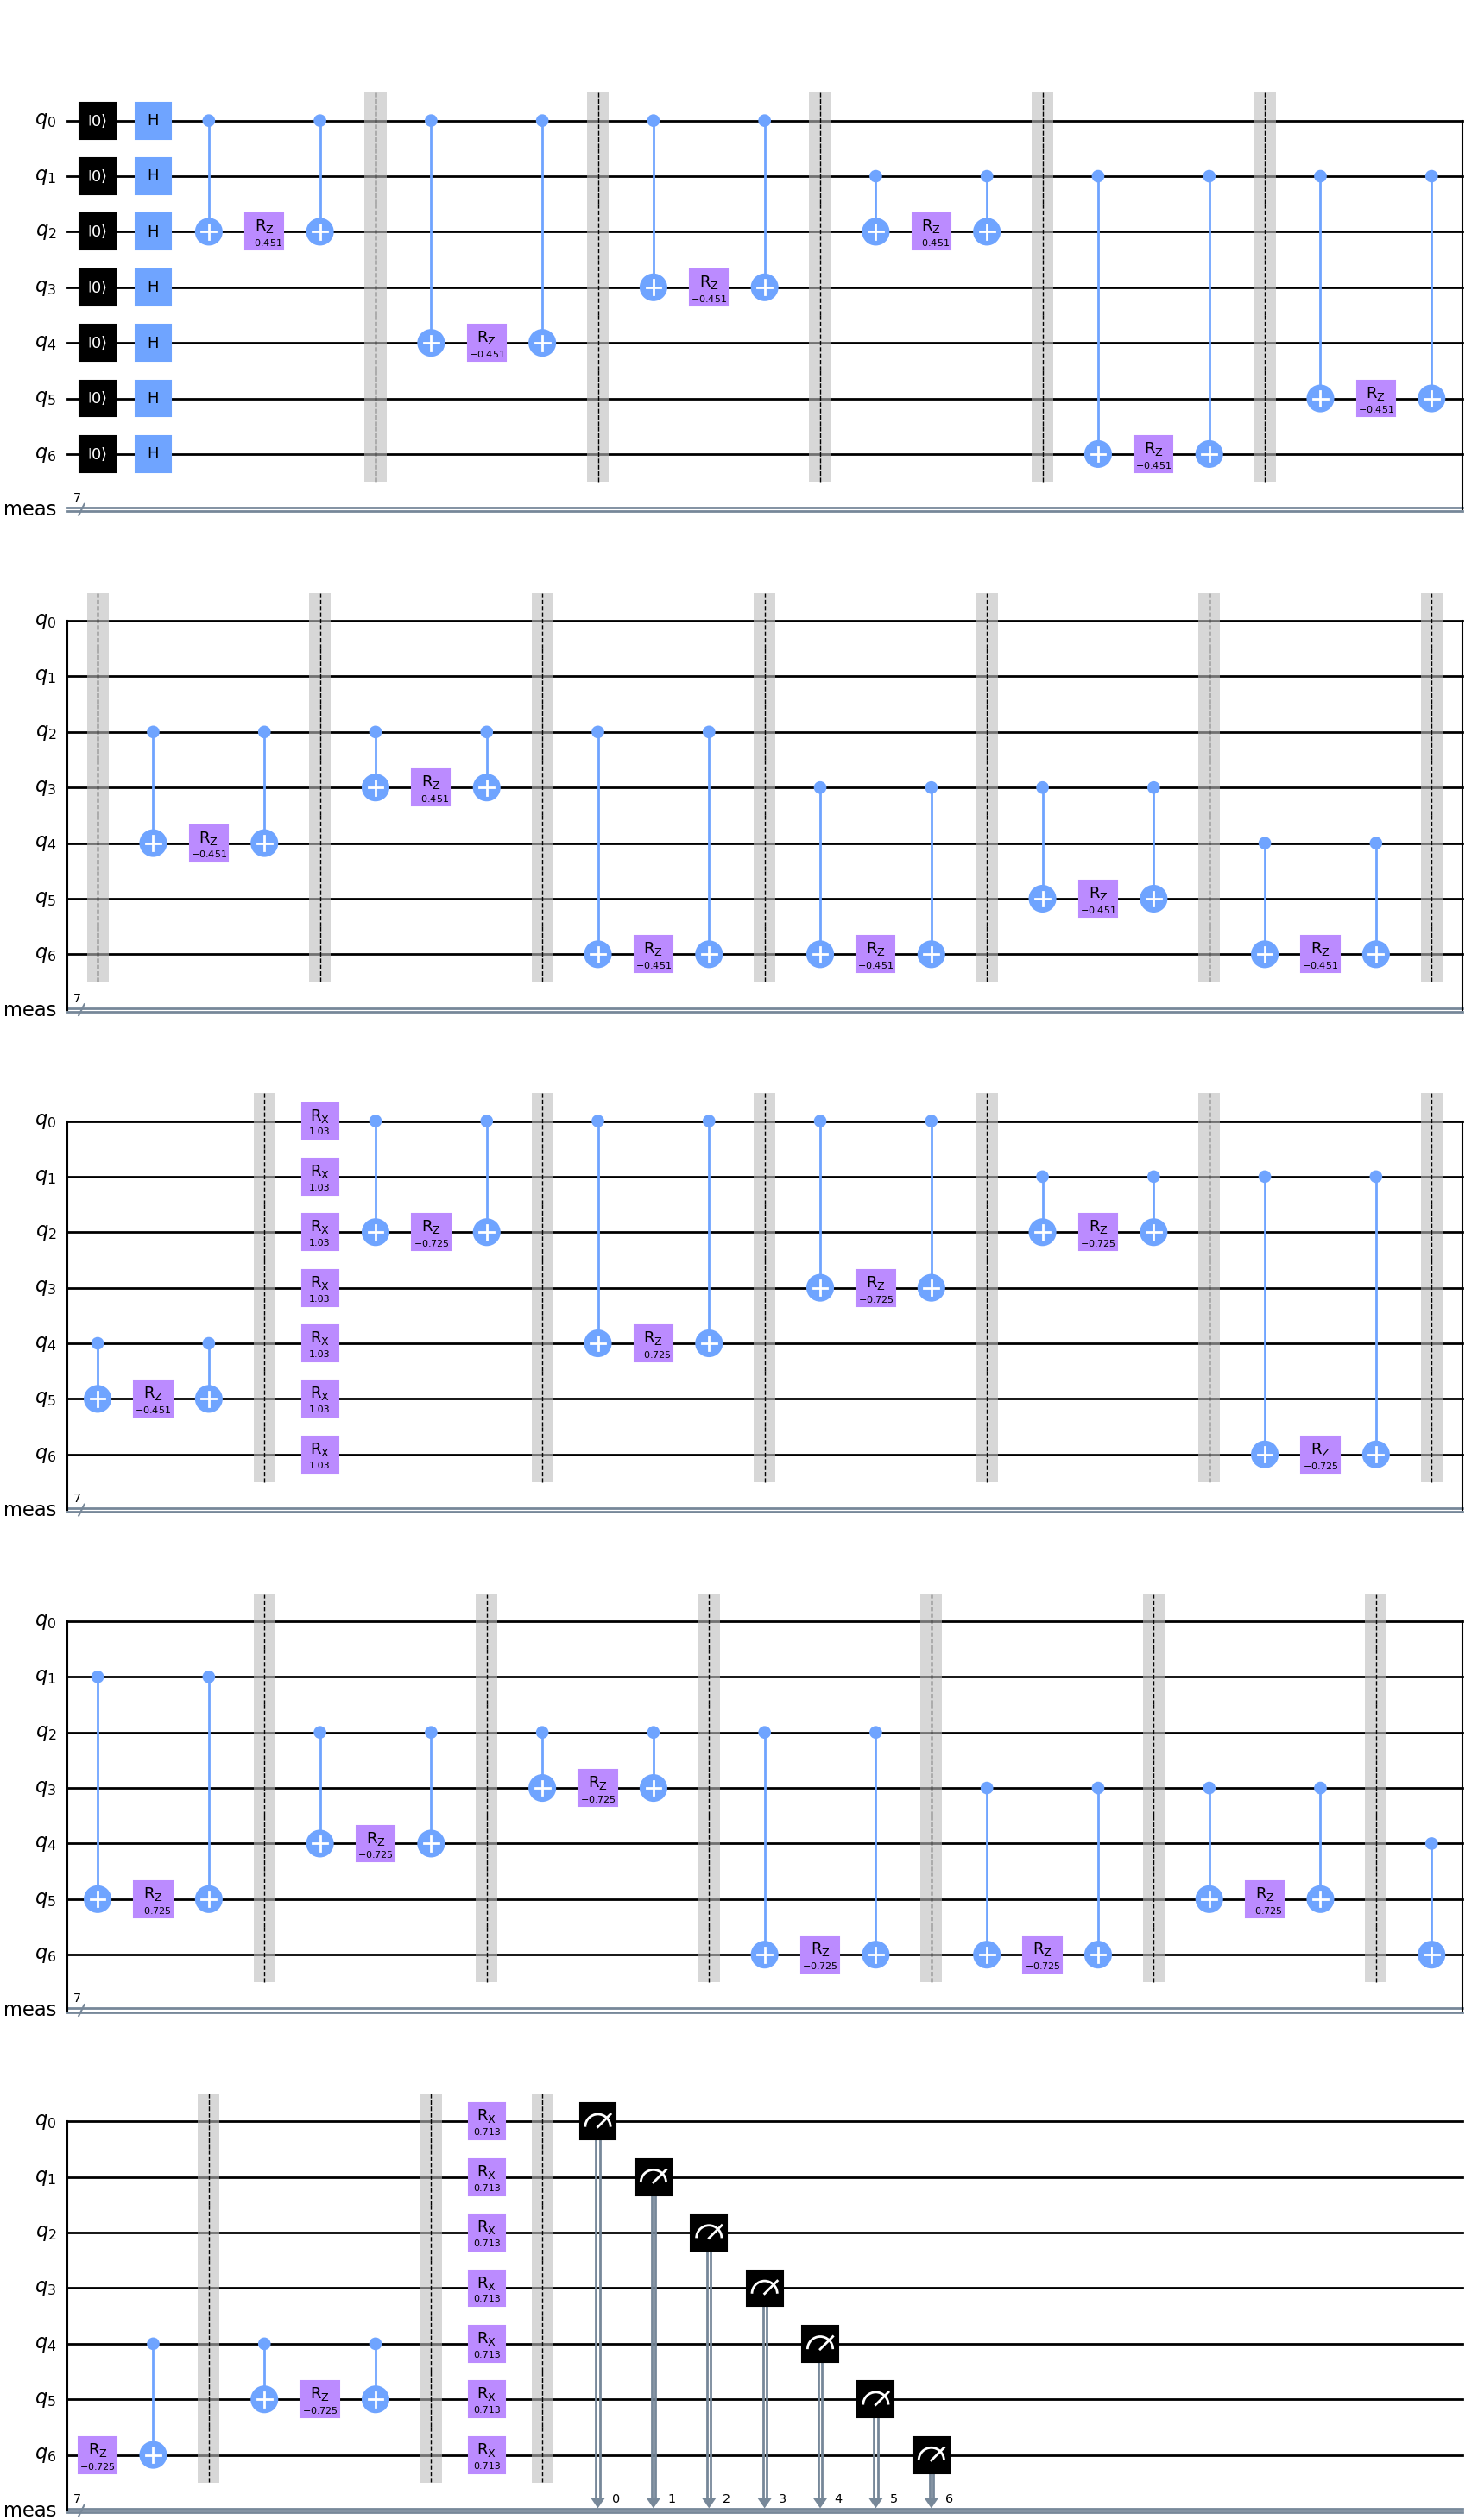
\includegraphics[width=0.3\textwidth]{circuit.png}
    \caption{A quantum circuit example at n=7,p=2.}
    \label{fig:example circuit}
\end{figure}

\begin{figure}[!htb]
    \centering
    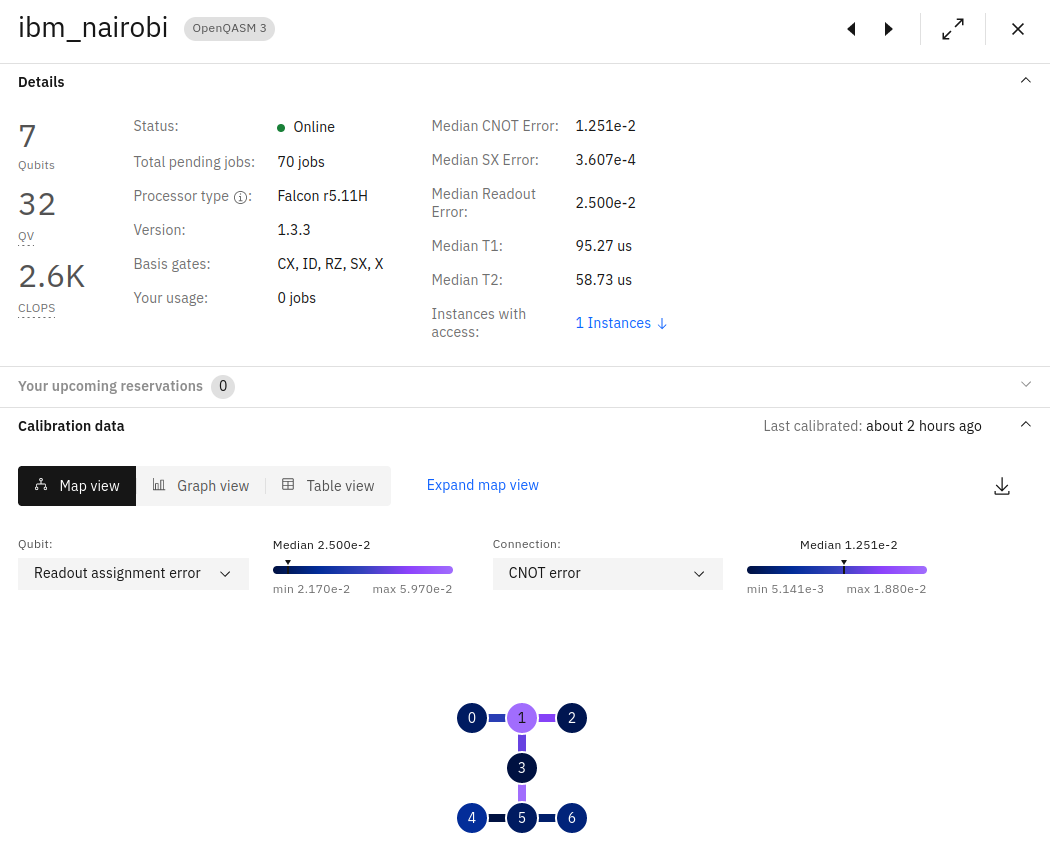
\includegraphics[width=0.42\textwidth]{overview of ibm_nairobi.png}
    \caption{Overview of IBM nairobi}
    \label{fig:overview of ibm_nairobi}
\end{figure}

\begin{figure}[!htb]
    \centering
    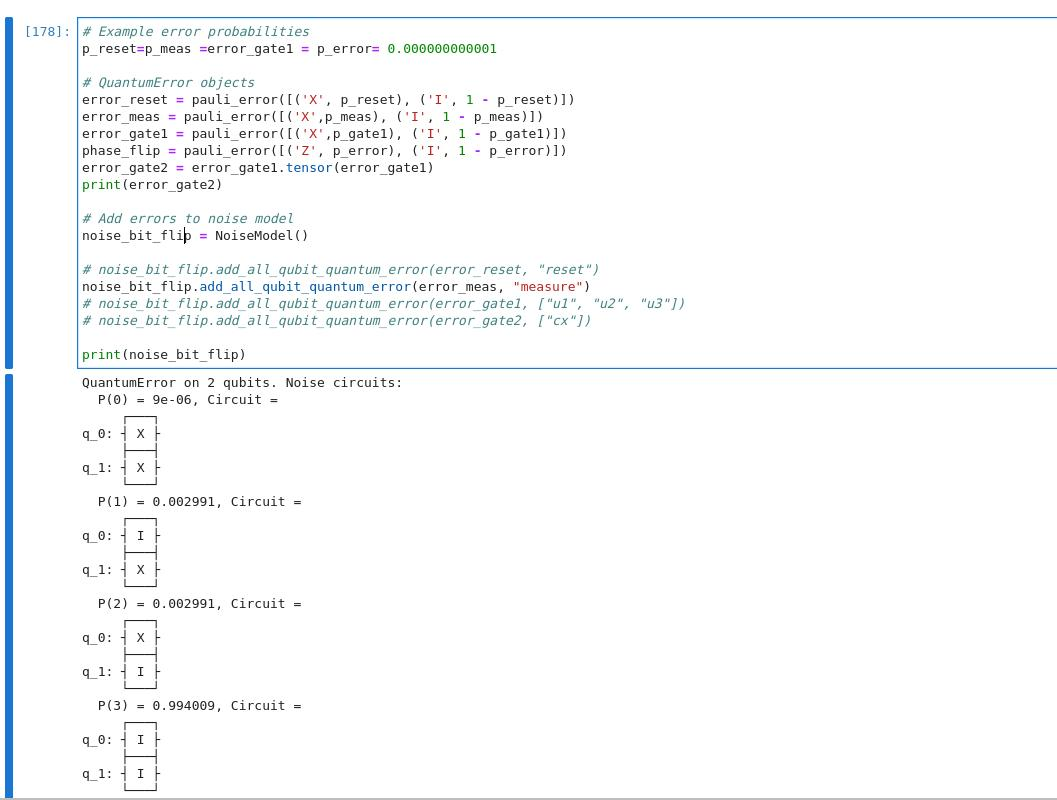
\includegraphics[width=0.3\textwidth]{failure.jpg}
    \caption{A Failed Attempt to Construct the $R_z$ Error}
    \label{fig:failure}
\end{figure}

We obtain our result both with and without noise with the help of \textbf{qasm\_simulator}. We draw the top 5 states of each situation in the same histogram for $p$ in $range(1,7)$. We try the original 1024 shots shown results in FIG.\ref{fig:1024-shots} and the large enough 100000 shots  shown results in FIG.\ref{fig:100000-shots}, which we aim to observe the real quantum computation result and the expectation of the final states individually. At the same time, we plot the Accuracy-p figure with and without noise, to help us better understand the influence of noise. 
\begin{align*}
    \text{Accuracy}=\frac{\text{number of desired states}}{\text{total shot number}}
\end{align*}

Besides, in the experiment, we attempt to construct the $R_z$ error ourselves, which turns out to be another \textbf{precision disaster}. As shown in the FIG.\ref{fig:failure}, we set the possibility of error to zero, but we still obtain an undesired gate result.It's $P(1)$ is obviously not 0 and its $P(3)$ is not 1. We failed to fix this precision bug. That's why we turn to actual quantum machine noise data.




\subsection{Experiment Design summary}
\begin{enumerate}
    \item We implement QAOA on Max-Cut using  a unitary matrix operator.
    \item We tried three different ways of parameter optimization and test them with various n and p to find out the pros and cons.
    \item We construct the quantum circuit of QAOA.
    \item We simulate the quantum circuit using qiskit and use real quantum machine's error data to simulate the noise.
    \item We plot our experiment result and discuss the reason behind it.
\end{enumerate}
\clearpage
\section{Experiment Result and Analyse}

\subsection{Comparison of different optimizor}

TABLE.\ref{tab:Opt} compares the performances of different optimizers on data with different attributes. It is shown that when $p=1, 2$, the result of brute force is relatively not bad. However, as $p$ increases, the brute force algorithm takes too long to execute and the Bayes algorithm meets difficulty in accuracy. BFGS algorithm remains the most stable one.

The result also shows that the accuracy grows significantly with $p$ when $p$ is not so large.

\begin{table}[htbp]
  \centering
  \caption{Optimizor}
    \begin{tabular}{lrrrrrr}
\toprule
          & \multicolumn{3}{c}{n=7, p=1, k=20} & \multicolumn{3}{c}{n=7, p=2, k=10} \\
\midrule
    real answer & 8     & 3     & 9     & 4     & 15    & 8 \\
    Bayes  & 6.299  & 2.357  & 7.271  & 3.384  & 13.209  & 6.274  \\
    BFGS  & 6.307  & 2.380  & 7.336  & 3.122  & 13.601  & 6.696  \\
    brute force & 6.140  & 2.337  & 7.213  & 3.343  & 11.860  & 6.043  \\
    BFGS ratio & 0.788  & 0.793  & 0.815  & 0.781  & 0.907  & 0.837  \\
\midrule
          & \multicolumn{3}{c}{n=7, p=3} & \multicolumn{3}{c}{n=7, p=4} \\
\midrule
    real answer & 12.000  & 8.000  & 11.000  & 15.000  & 14.000  & 13.000  \\
    Bayes  & 9.933  & 5.693  & 8.154  &       &       &  \\
    BFGS  & 11.100  & 6.698  & 9.218  & 14.041  & 12.726  & 11.817  \\
    BFGS ratio & 0.925  & 0.837  & 0.838  & 0.936  & 0.909  & 0.909  \\
\bottomrule
    \end{tabular}%
   \label{tab:Opt}%
\end{table}%

\subsection{Parameter Optimization}
We are interested in how the $F_p$ of a certain graph develops as p grows.

\begin{figure}[!htb]
    \centering
        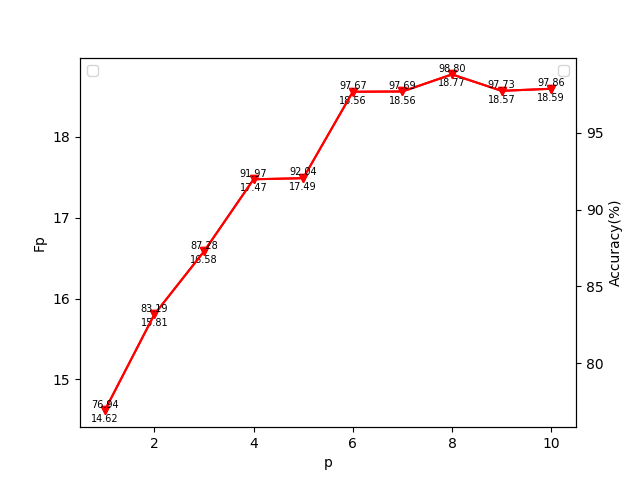
\includegraphics[width=0.4\textwidth]{pic/result_8.png}
        \caption{The relationship between $F_p$ and $p$ , $n=8$}
    \label{fig:result_8}
\end{figure}

First, we run our algorithm at n=8, shown as FIG.\ref{fig:n=8} and we got the result as FIG.\ref{fig:n=8}. For p larger than 6, we achieve an accuracy of 97\%, which is impressive. Some fluctuation occurs when p is large. It's because our optimization algorithm may have stuck in the local minima sometimes. 

Then, we run our algorithm at n=7, shown as FIG.\ref{fig:n=7} and we got the result as FIG.\ref{fig:n=7}. We even achieve an accuracy of 99.86\%! Since n is smaller, we got a smooth monotonically increasing curve this time.
\begin{figure}[!htb]
    \centering
        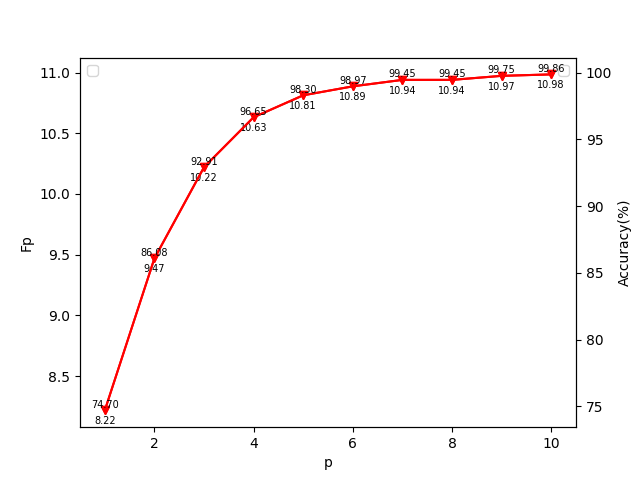
\includegraphics[width=0.4\textwidth]{pic/result_7.png}
        \caption{The relationship between $F_p$ and $p$ on the fixed graph with $n=7$ vertices}
    \label{fig:result_7}
\end{figure}


Besides, it's worth mentioning that since p refers to the time our edges could expand to its neighbors, the longest path in the solution graph at $p$ is $2p+1$\cite{farhi2014quantum}, which means the final solution may be unachievable for small p in theory. 

In conclusion, the experiment result shows that $F_p$ increases as $p$ increases and 
\begin{align*}
    \lim_{p\rightarrow \infty}\max_{\vec{\gamma}, \vec{\beta}}{F_p(\vec{\gamma}, \vec{\beta})}=C_{max}(z)
\end{align*}







\subsection{Quantum Circuits Simulation}


The top-5 quantum circuit's result states histogram pictures are shown in FIG.\ref{fig:1024-shots} and FIG.\ref{fig:100000-shots}, 1024 shots situation and 100000 shots situation correspondingly.
%\clearpage
\begin{figure*}[!htb]
    \centering
    \subfloat[1024 shots]{
        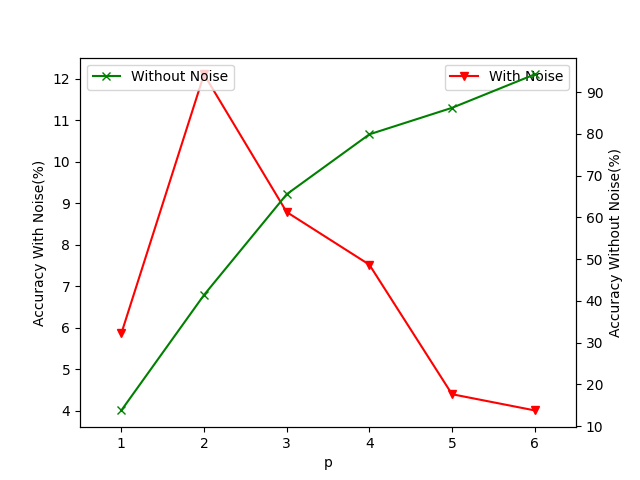
\includegraphics[width=0.42\textwidth]{result/[shots=1024]Accuracy-P}
    }
    \subfloat[100000 shots]{
        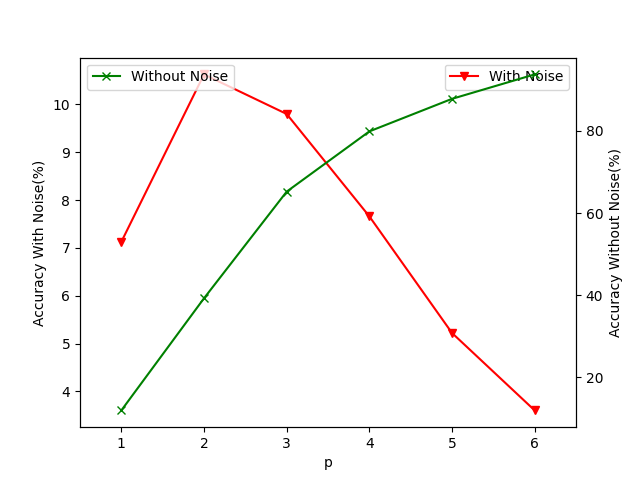
\includegraphics[width=0.42\textwidth]{result/Accuracy-P}
    }
    \caption{Accuracy-P digram}
    \label{fig:Accuracy-P}
\end{figure*}

\begin{figure*}[!htb]
    \centering
    \begin{minipage}{\textwidth}
        \centering
        \subfloat[$P=1$]{
            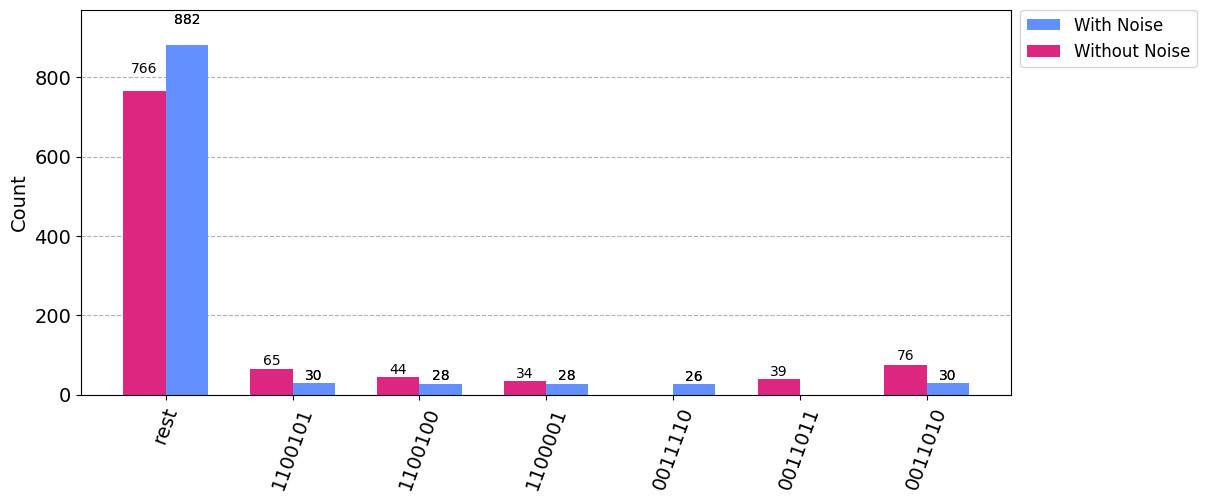
\includegraphics[width=0.3\textwidth]{result/[shots=1024]P=1}
        }
        \subfloat[$P=2$]{
            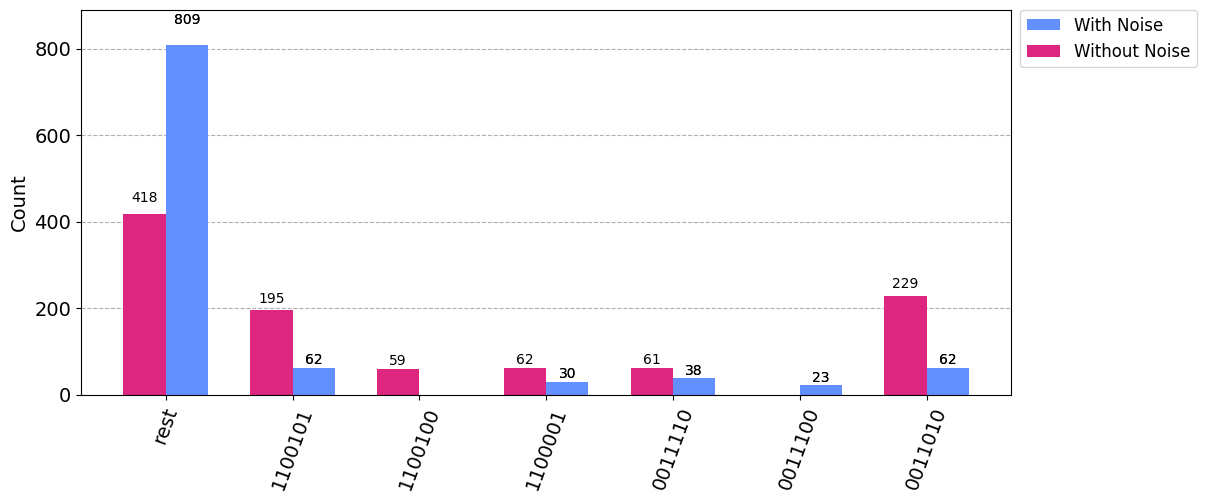
\includegraphics[width=0.3\textwidth]{result/[shots=1024]P=2}
        }
        \subfloat[$P=3$]{
            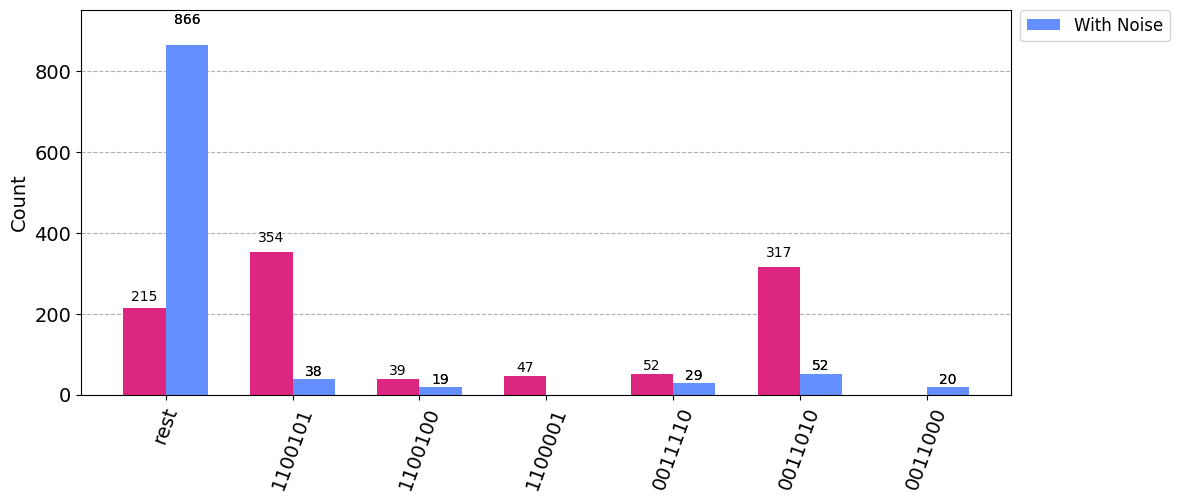
\includegraphics[width=0.3\textwidth]{result/[shots=1024]P=3}
        }
    
        \subfloat[$P=4$]{
            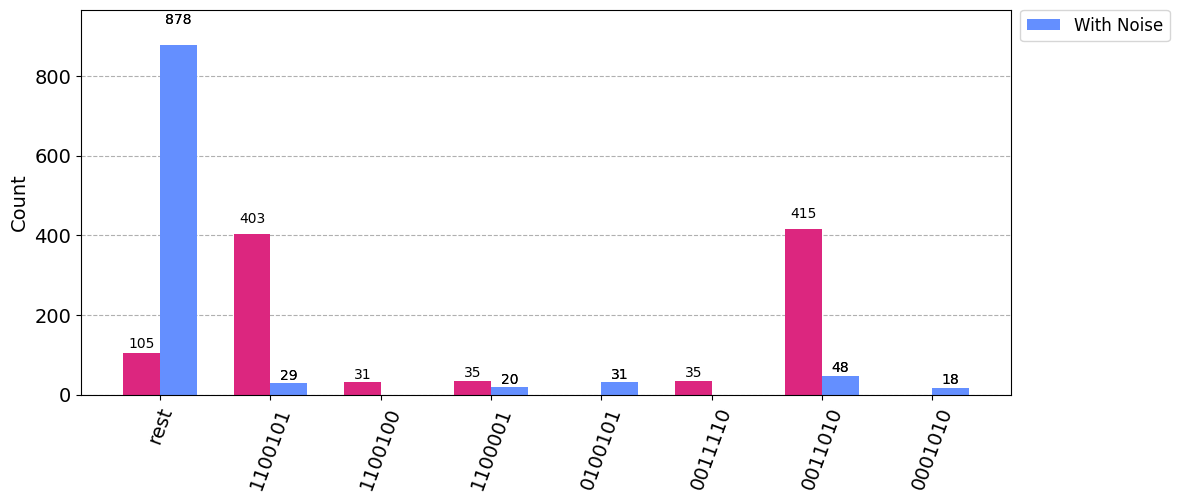
\includegraphics[width=0.3\textwidth]{result/[shots=1024]P=4}
        }
        \subfloat[$P=5$]{
            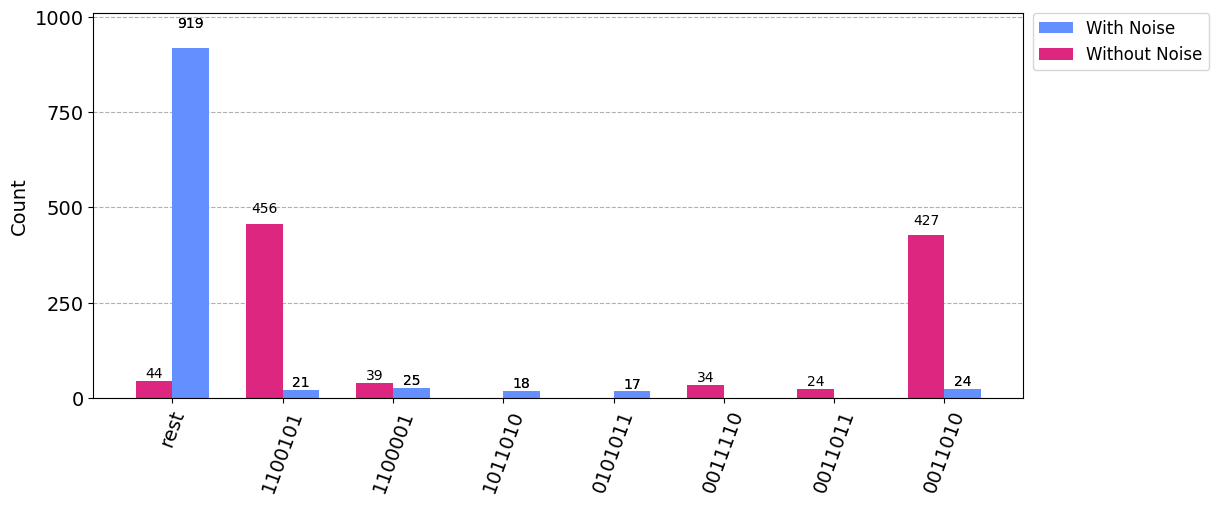
\includegraphics[width=0.3\textwidth]{result/[shots=1024]P=5}
        }
        \subfloat[$P=6$]{
            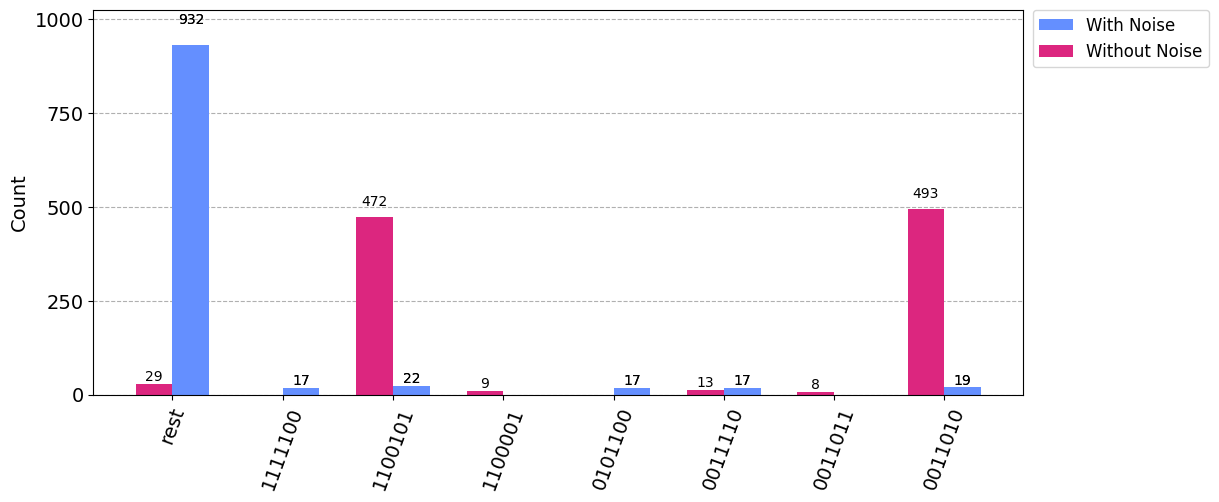
\includegraphics[width=0.3\textwidth]{result/[shots=1024]P=6}
        }
        \caption{Output states statistics for different p at 1024 shots}
        \label{fig:1024-shots}
    \end{minipage}

    \begin{minipage}{\textwidth}
        \centering
        \subfloat[$P=1$]{
            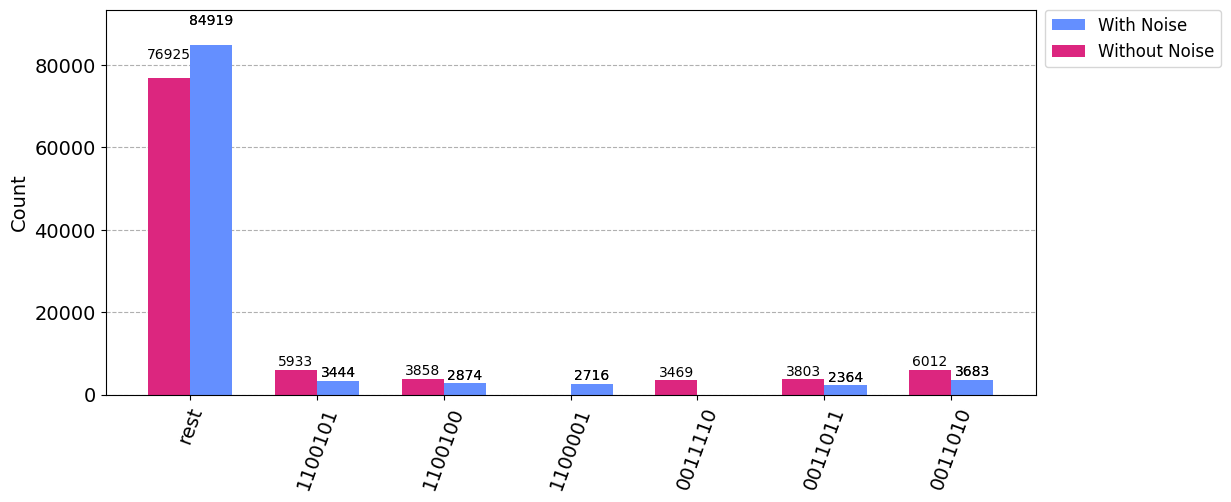
\includegraphics[width=0.3\textwidth]{result/P=1}
        }
        \subfloat[$P=2$]{
            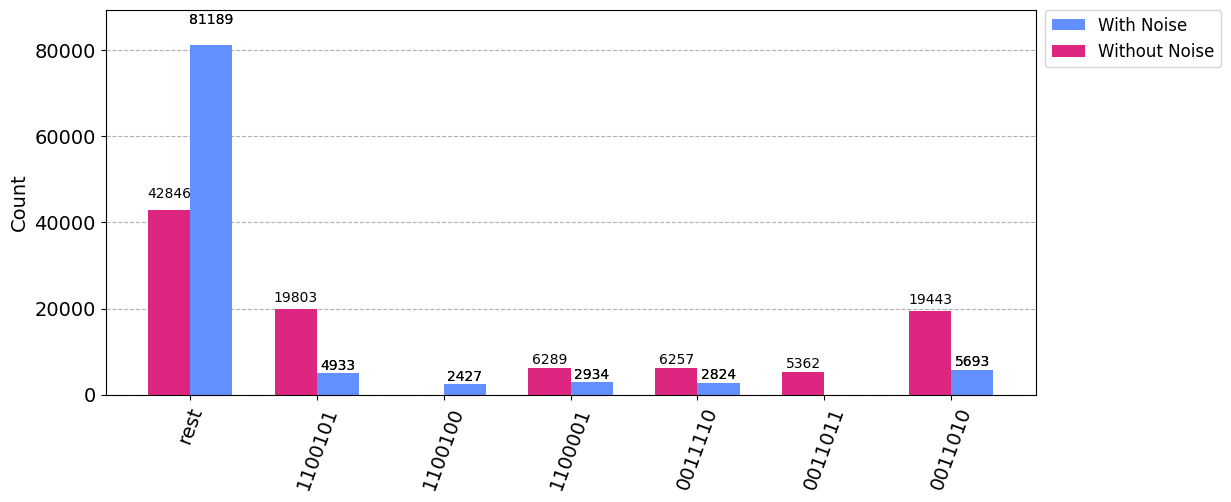
\includegraphics[width=0.3\textwidth]{result/P=2}
        }
        \subfloat[$P=3$]{
            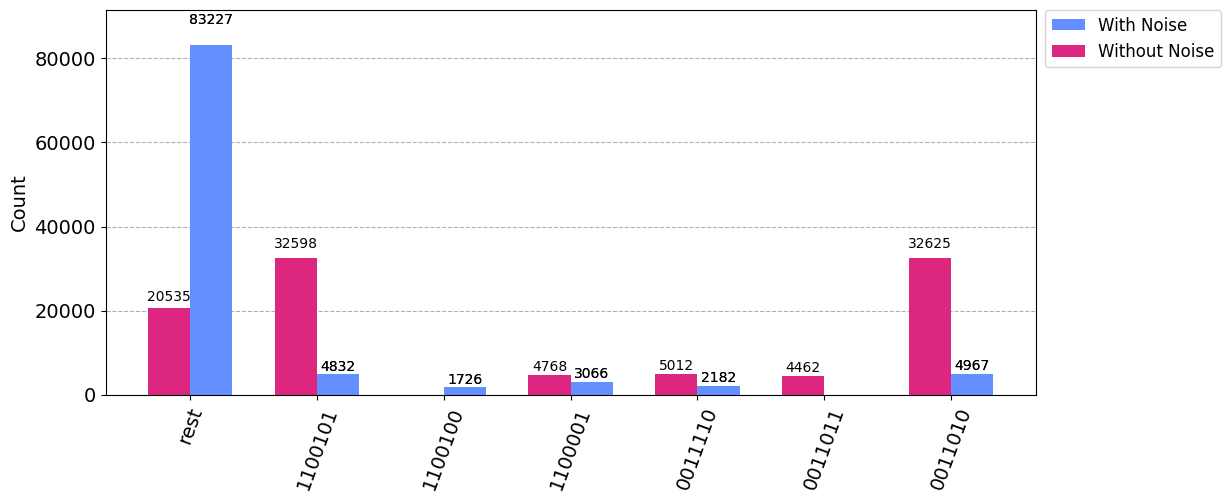
\includegraphics[width=0.3\textwidth]{result/P=3}
        }
    
        \subfloat[$P=4$]{
            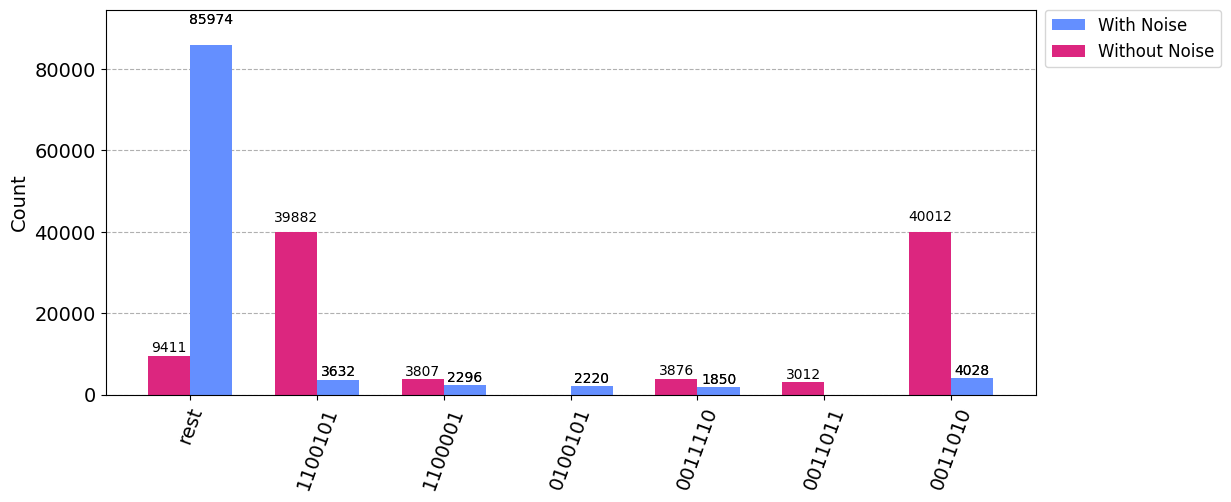
\includegraphics[width=0.3\textwidth]{result/P=4}
        }
        \subfloat[$P=5$]{
            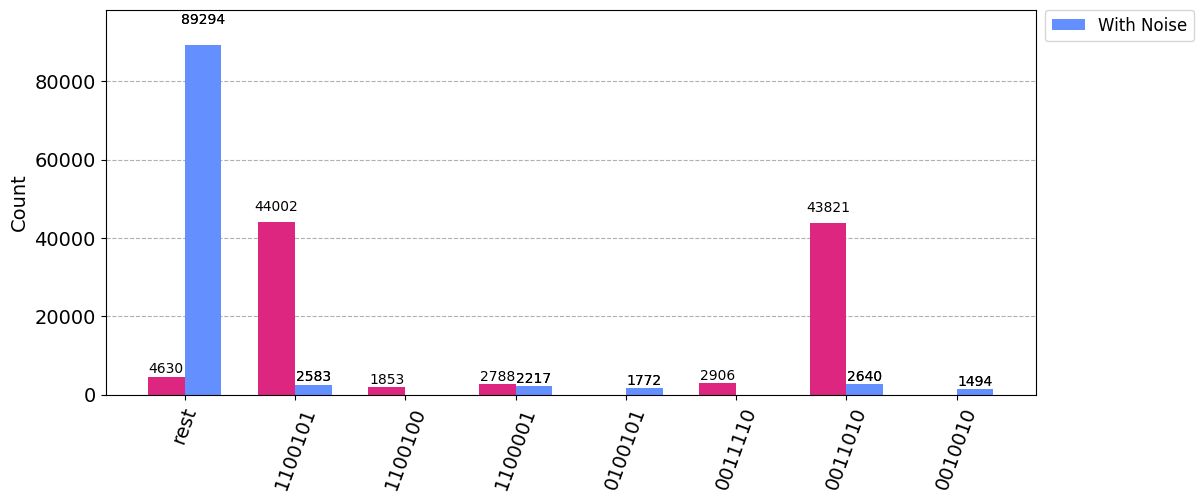
\includegraphics[width=0.3\textwidth]{result/P=5}
        }
        \subfloat[$P=6$]{
            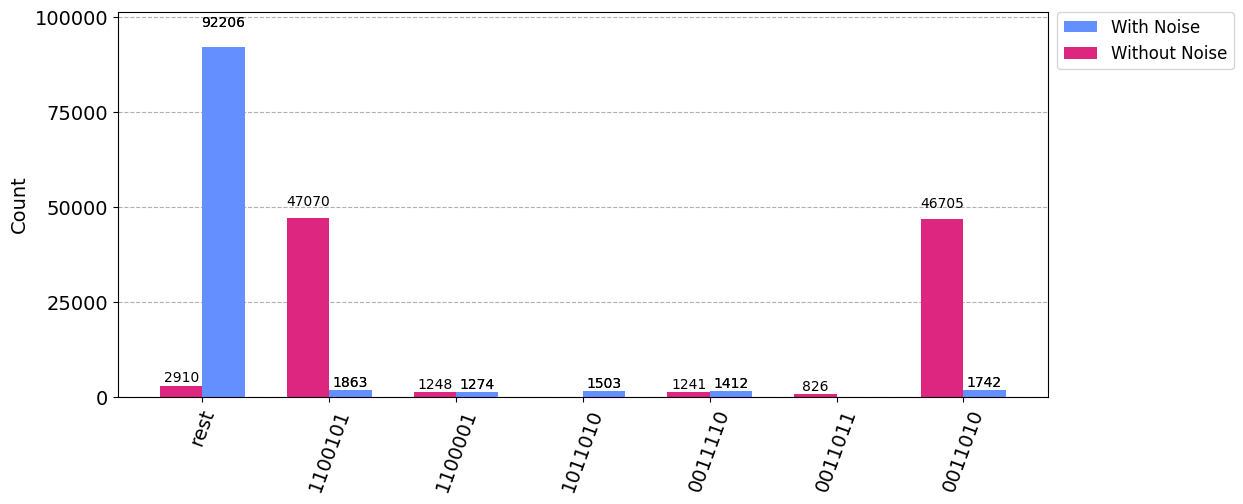
\includegraphics[width=0.3\textwidth]{result/P=6}
        }
        \caption{Output states statistics for different p at 100000 shots}
        \label{fig:100000-shots}
    \end{minipage}
\end{figure*}
\clearpage
We will find that for shots=100000 in FIG.\ref{fig:Accuracy-P}, the accuracy states could always be distinguished, though hard. So the noise only decreases the possibility of our desired states  and randomly attributes them with other states. Since the same process act on every state, the possibility of our desired states is still ahead of others, though the gap is getting smaller as the depth of the quantum circuit increase.

However, for shots=1024, they could only be figured out at $p=2$ and 3. It's due to the random nature of quantum measurement. As long as the expectation two states are close, they will mix up easily. So in practice, we must control the depth of the quantum circuit since the random nature of quantum measurement may bridge the gap between our desired states and others.

As we analyze the Accuracy-p figure in FIG.\ref{fig:1024-shots} and  FIG.\ref{fig:100000-shots}, it's easy to obtain that noise dramatically decreases the accuracy. As $p$ increases, the depth of the quantum circuit increases, leading to more noise and less accuracy. 

Besides, although  accuracy increases with $p$ for noiseless situations just as it's theoretically proved, the noise effect will overweigh the accuracy improvement of $p$ and become dominant for a sufficiently large $p$ (in this case $p=2$). That's why accuracy first increases and then decreases as $p$ increases.

So we should carefully choose our p when we deploy QAOA in the real quantum machine.




% \begin{figure*}[!htbp]
%     \centering
%     \subfloat[$P=1$]{
%         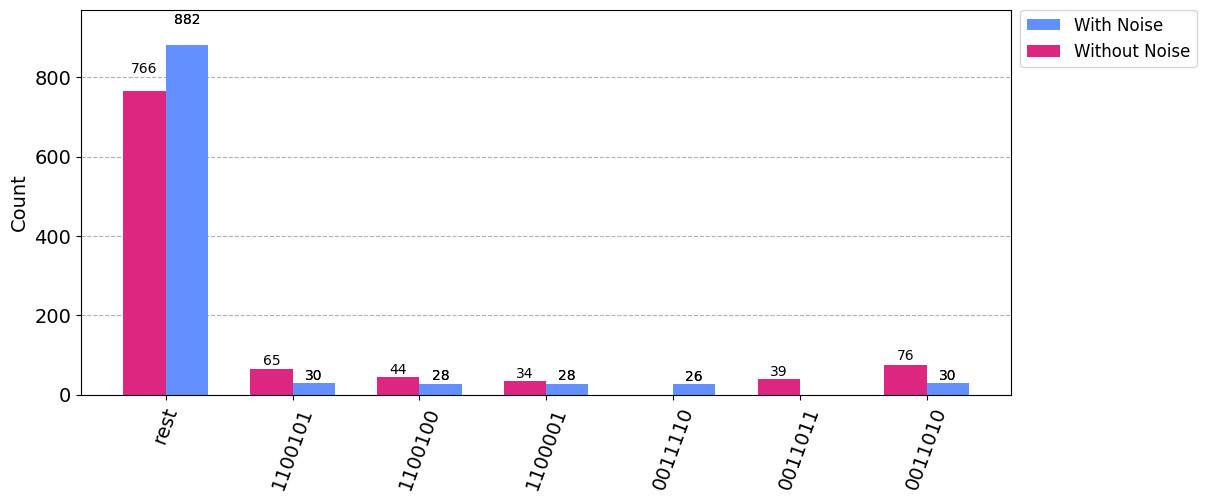
\includegraphics[width=0.5\textwidth]{result/[shots=1024]P=1}
%     }
%     \subfloat[$P=2$]{
%         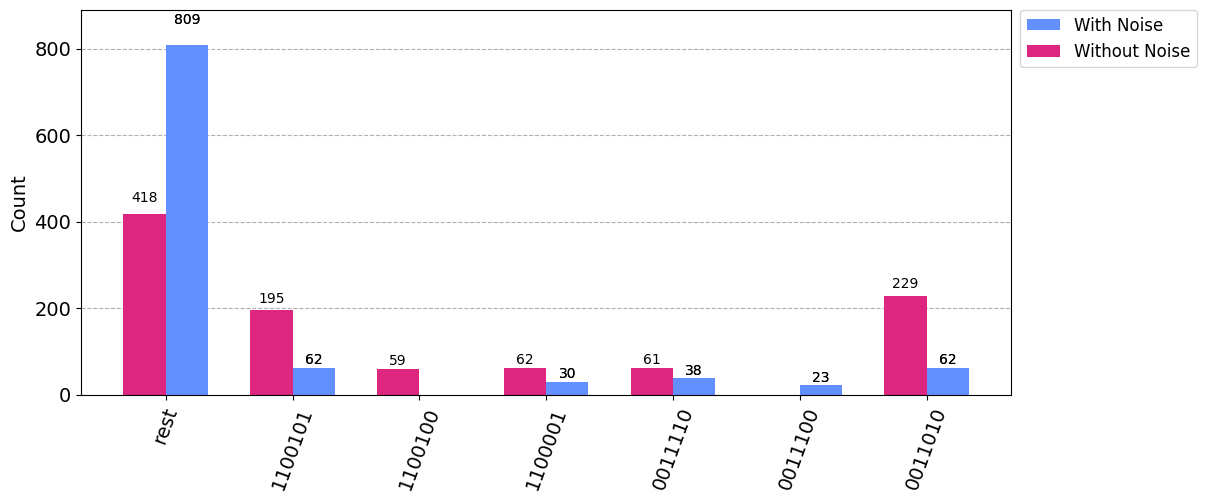
\includegraphics[width=0.5\textwidth]{result/[shots=1024]P=2}
%     }
    
%     \subfloat[$P=3$]{
%         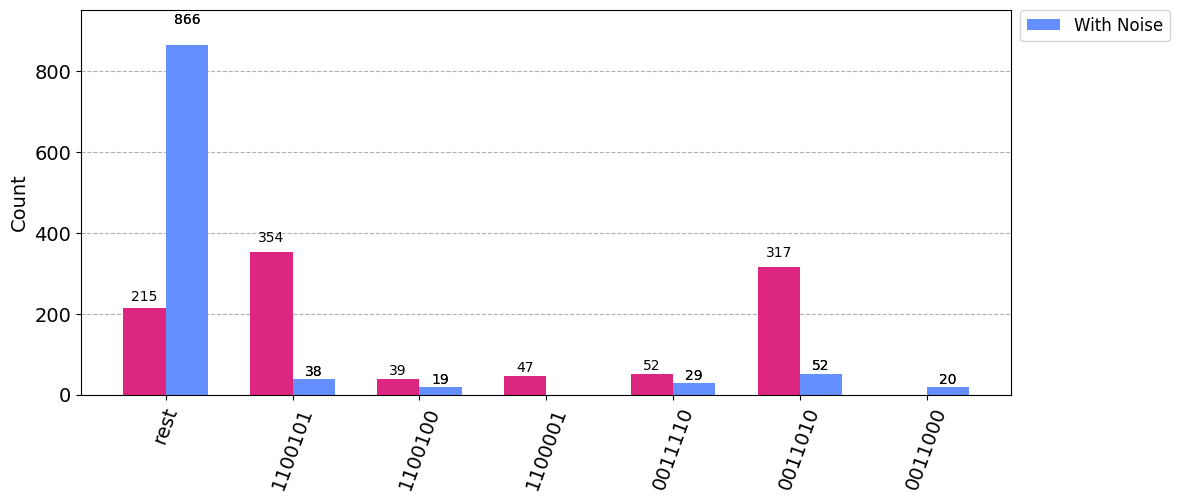
\includegraphics[width=0.5\textwidth]{result/[shots=1024]P=3}
%     }
%     \subfloat[$P=4$]{
%         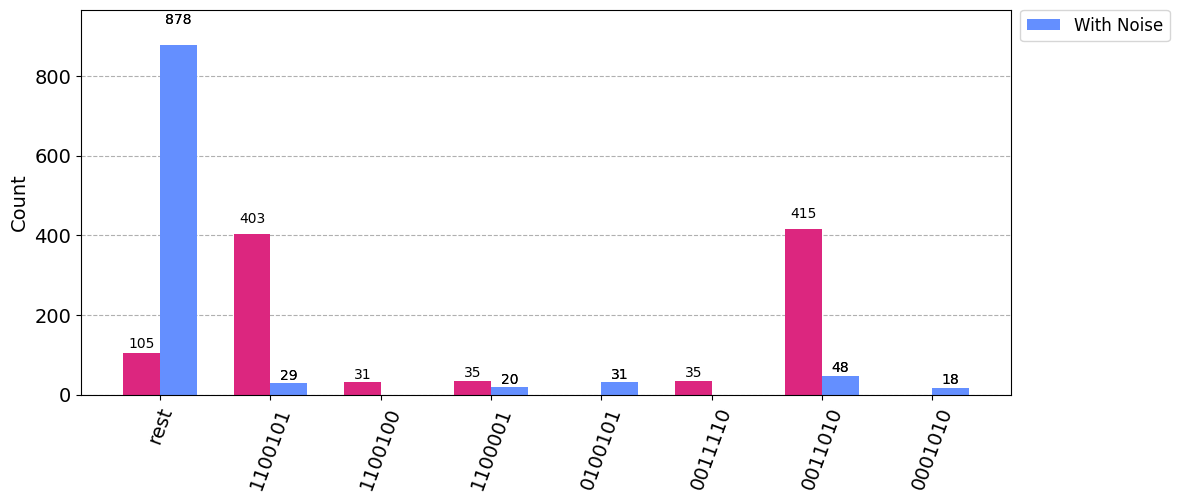
\includegraphics[width=0.5\textwidth]{result/[shots=1024]P=4}
%     }
    
%     \subfloat[$P=5$]{
%         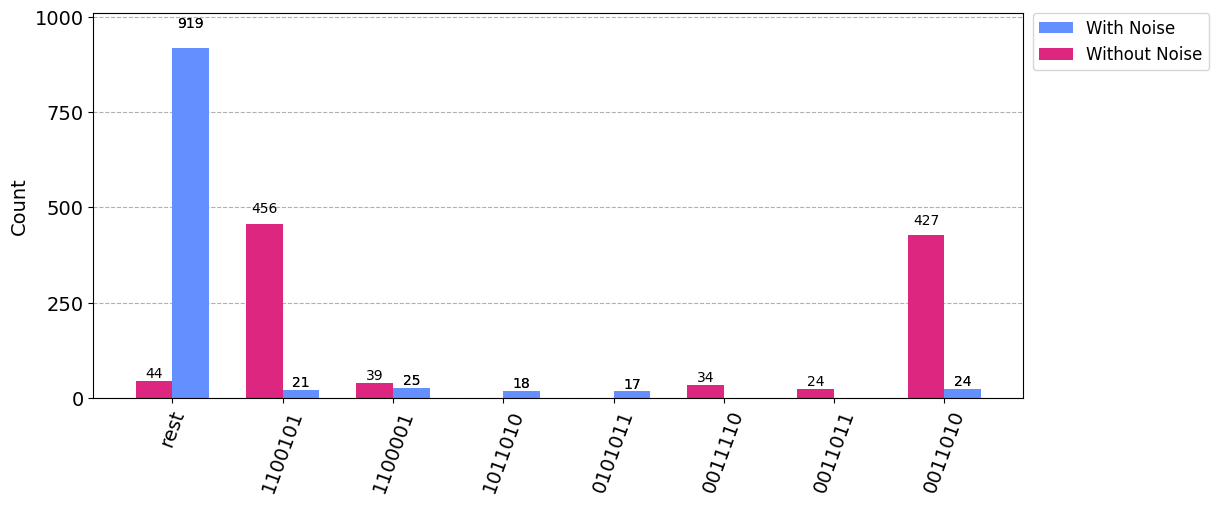
\includegraphics[width=0.5\textwidth]{result/[shots=1024]P=5}
%     }
%     \subfloat[$P=6$]{
%         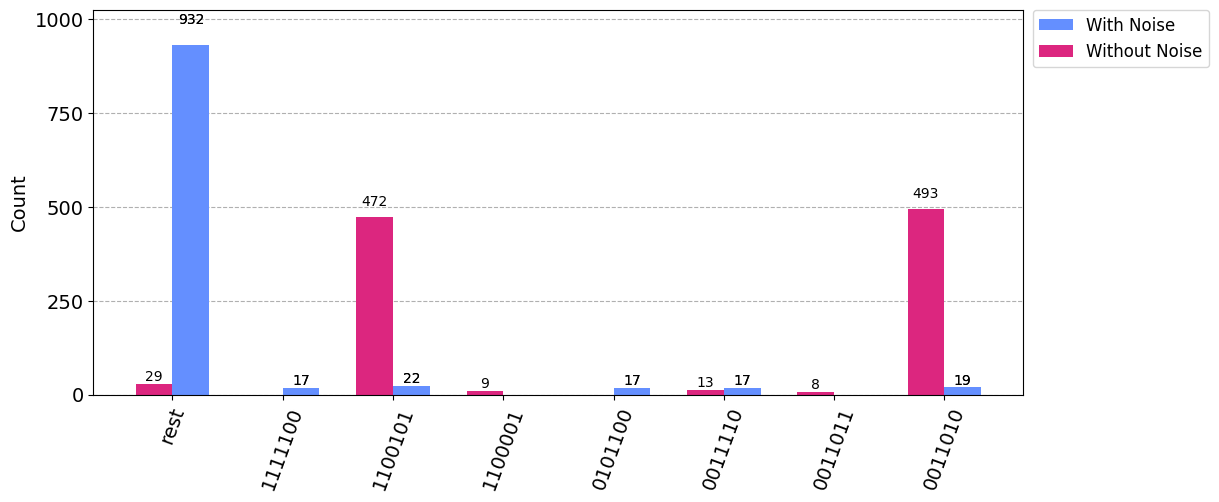
\includegraphics[width=0.5\textwidth]{result/[shots=1024]P=6}
%     }
%     \caption{1024 shots}
%     \label{fig:1024-shots}
% \end{figure*}

% \begin{figure*}[!htbp]
%    \centering
%     \subfloat[$P=1$]{
%         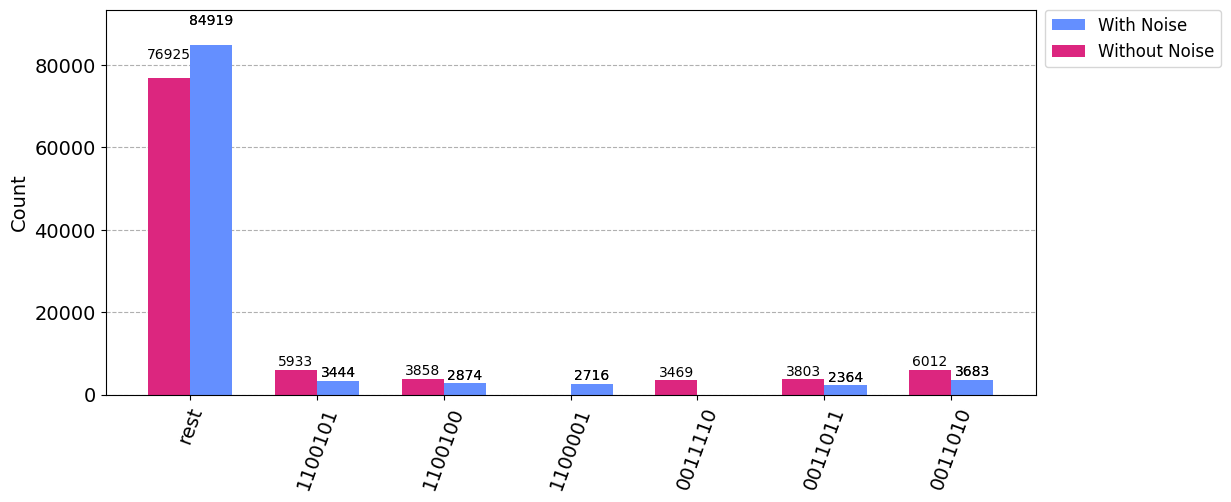
\includegraphics[width=0.5\textwidth]{result/P=1}
%     }
%     \subfloat[$P=2$]{
%         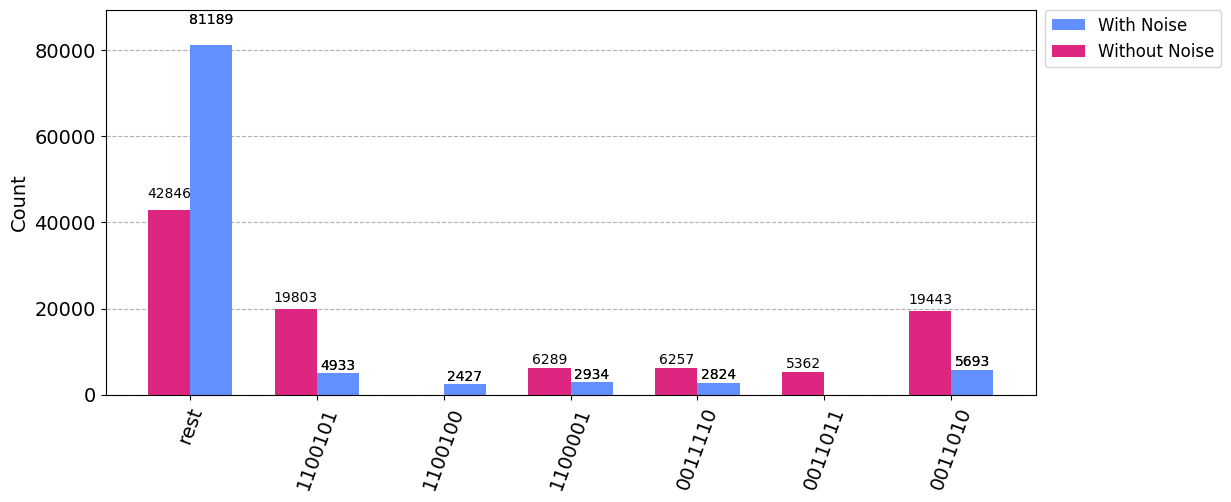
\includegraphics[width=0.5\textwidth]{result/P=2}
%     }
    
%     \subfloat[$P=3$]{
%         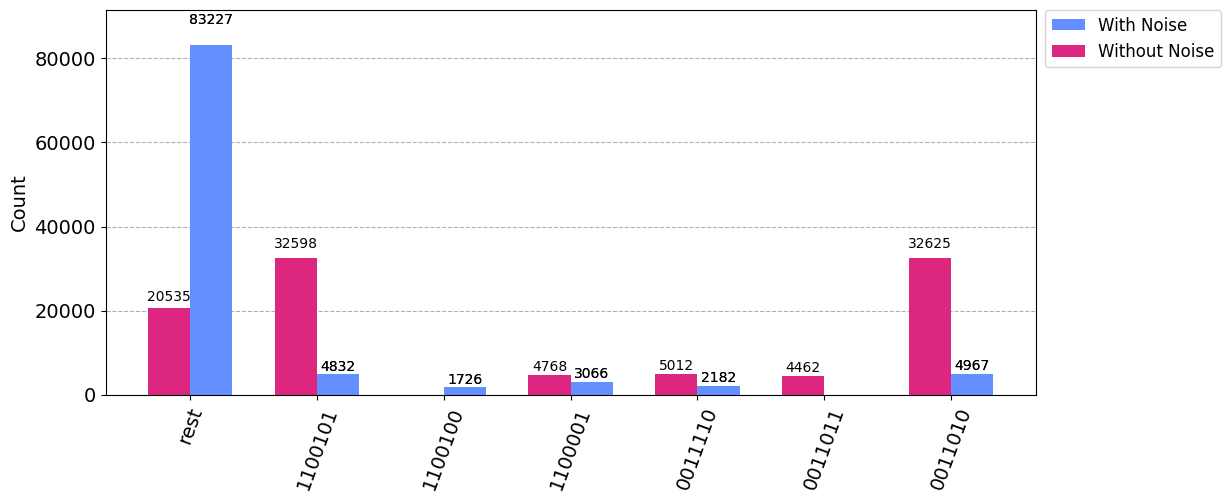
\includegraphics[width=0.5\textwidth]{result/P=3}
%     }
%     \subfloat[$P=4$]{
%         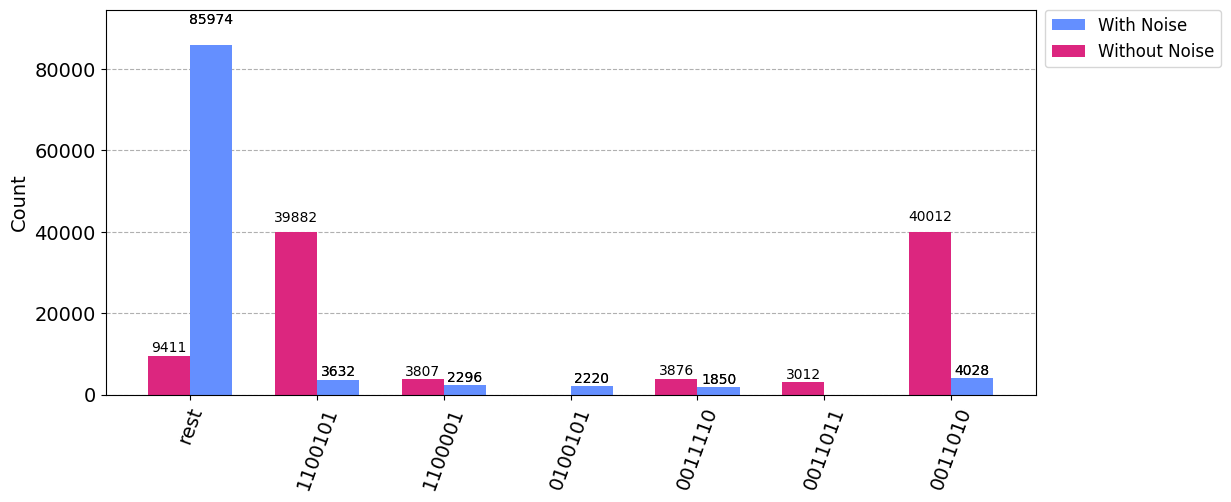
\includegraphics[width=0.5\textwidth]{result/P=4}
%     }
    
%     \subfloat[$P=5$]{
%         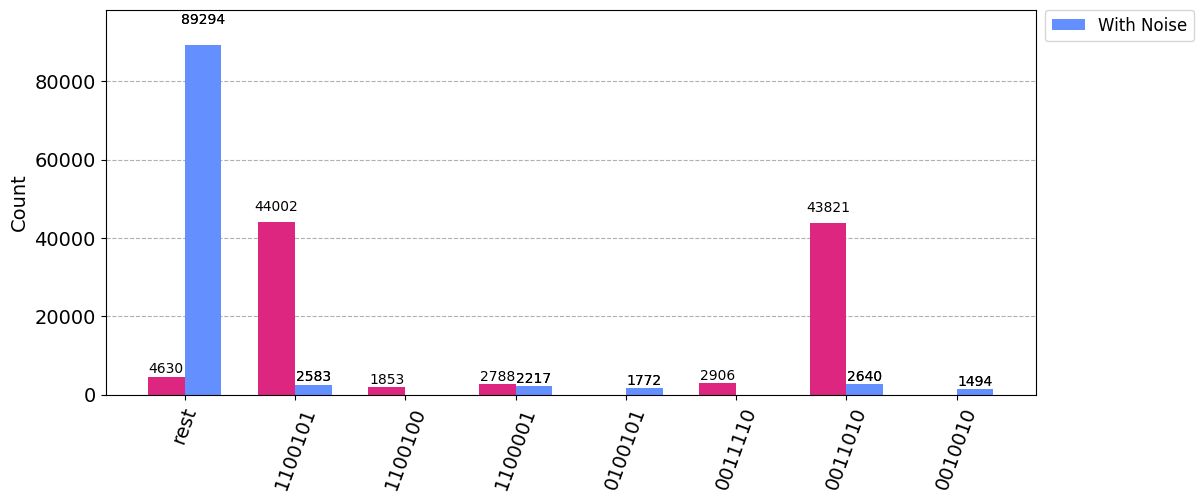
\includegraphics[width=0.5\textwidth]{result/P=5}
%     }
%     \subfloat[$P=6$]{
%         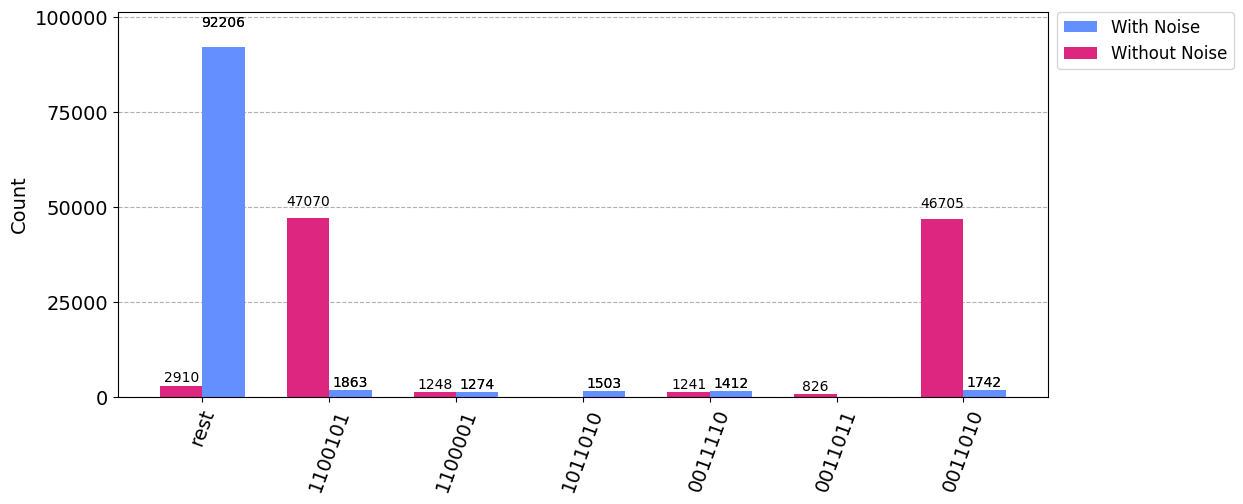
\includegraphics[width=0.5\textwidth]{result/P=6}
%     }
%     \caption{100000 shots}
%     \label{fig:100000-shots}
% \end{figure*}

%\clearpage

\section{Conclusion}

\subsection{Our Achievement}
Quantum Approximate Optimization Algorithm is a hybrid quantum-classical algorithm for solving combinatorial optimization problems. We studied the principle and procedure of this algorithm in comparison with QAA, understood how the parameters work in this algorithm, and learned the circuit representation of each involved operator.

Then we design abundant experiments and deploy it using Python. Our codes are available at  \href{https://github.com/qyy2003/QAOA}{https://github.com/qyy2003/QAOA}

\begin{enumerate}
    \item We implement unitary matrix operator simulation with two methods, eigenvalue decomposition and expm direct calculation, and fixed a precision disaster.
    \item We deploy three methods, grid search, Bayesian optimization and  basin-hopping trick supported L-BFGS-B algorithm, to optimize $\vec{\gamma}, \vec{\beta}$ optimization and compare their performances. It turns out that gradient-based algorithms,  L-BFGS-B in particular, have done a way better job.
    \item We study the quantum circuits construction theory and implement it with qiskit SDK, which could be run on real quantum machines. And we test our quantum circuits' performance both with and without noise. To better emulate the real noise, we use the data of a real IBM  Quantum Machines \textit{ibm\_nairob}. Then we analyze the influence of noise in different circumstances.
    \item  We study the influence of $p$ on QAOA for a given graph. Experiment results show that $F_p$ increases as $p$ grows and some fluctuation may occur due to the limitation of the optimization algorithm. Our noiseless experiments prove that
    \begin{align*}
    \lim_{p\rightarrow \infty}\max_{\vec{\gamma}, \vec{\beta}}{F_p(\vec{\gamma}, \vec{\beta})}=C_{max}(z)
    \end{align*}
    We discuss the influence of $p$ on output states both with and without noise and try some reasoning. 
    Neither too large nor too small, suitable $p$ is needed to achieve better results, according to our experiment.
\end{enumerate}

\subsection{Outlook}

\begin{itemize}
    \item In our work, the optimizers are based on noise-free simulators. The optimized parameters are then passed to a noisy environment in quantum computers to test their performance. However, in real applications, how to optimize the parameters in a noisy environment remains a large problem to solve.
    \item QAOA is a quantum computing method to replace classical algorithms. In our work, 
we dug into the performance of QAOA in different depth and using various optimizers, 
but haven't made a reasonable comparison between QAOA and state-of-art classical algorithms to show 
how quantum advantage appear in this field. This sort of work requires wider research on 
relative methods. 
    \item It was shown in our work that noise can greatly reduce the algorithm's 
performance and that the qubit we need is proportional to vertex number $n$. It remains to explore how 
to use as few qubits as possible to obtain similar performances as well 
as how to reduce the influence of environmental noise and detect the internal error.
\end{itemize}


\appendix

\section{Code}

\lstinputlisting[title={sim.py}, language=python]{code/sim.py}
\lstinputlisting[title={optimize.py}, language=python]{code/optimize.py}
\lstinputlisting[title={optimize.ipynb}, language=python]{code/opt.py}


\nocite{*}

\bibliography{references}


\end{document}
